%\documentclass{fhnwreport} %
%\usepackage[ngerman]{babel}
%\usepackage[T1]{fontenc}
%\usepackage[latin1]{inputenc}
%\usepackage{tikz}
%\usepackage{amsmath}
%\usetikzlibrary{arrows}
%\usepackage{lmodern}   %Type1-Schriftart f�r nicht-englische Texte 
%
%\usepackage{listings}
%\lstset{language=Matlab}
%
%\usepackage{color}

%% Farben f�r Matlab-Listings
%\definecolor{hellgelb}{rgb}{1,1,0.85}     % Hintergrundfarbe
%\definecolor{colKeys}{RGB}{0,0,255}       % blau
%\definecolor{colIdentifier}{RGB}{0,0,0}	  % schwarz
%\definecolor{colComments}{RGB}{34,139,34} % gruen
%\definecolor{colString}{RGB}{160,32,240}  % violett
%
%\lstset{%
    %language=Matlab,%
    %%backgroundcolor={\color{hellgelb}},%
		%backgroundcolor={},%
    %basicstyle={\footnotesize\ttfamily},%
    %breakautoindent=true,%
    %breakindent=10pt,%
    %breaklines=true,%
    %captionpos=t,%
    %columns=fixed,%
    %%commentstyle={\itshape\color{colComments}},%
		%commentstyle={\color{colComments}},
    %extendedchars=true,%
    %float=hbp,%
    %frame=single,%
    %framerule=1pt,%
    %identifierstyle={\color{colIdentifier}},%
    %keywordstyle={\color{colKeys}},%
    %numbers=left,%
    %numbersep=1em,%
    %numberstyle={\tiny\ttfamily},%
    %showspaces=false,%
    %showstringspaces=false,%
    %stringstyle={\color{colString}},%
    %tabsize=4,%
    %xleftmargin=1em,%
    %xrightmargin=1em%
%} 
%\graphicspath{{./PrettyPictures}} 
%
%\begin{document}
\section{Elektrotechnische Probleml�sung}\label{ETProblemsolving}
In diesem Kapitel wird das Vorgehen zur Elektrotechnischen Probleml�sung genauer erl�utert. Dabei wird n�her auf die Grundlagen der Regelungstechnik, die Zellweger-Methode, einige Faustformeln und das Berechnen des geschlossenen Regelkreises eingegangen.

\subsection{Regelungstechnische Grundlagen}\label{RegelGrundlagen}
Ein Regelkreis besteht aus einer Strecke und einem Regler.

\begin{figure}[h]%Bild eines gesamten Regelkreises(Wikipedia):http://de.wikipedia.org/wiki/Regelkreis#/media/File:Einfacher_Regelkreis_n.svg
\centering
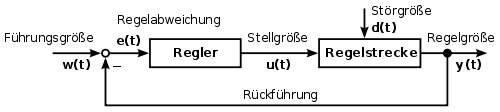
\includegraphics[width=0.8\textwidth]{./Einfacher_Regelkreis_Wikipedia.png}
\caption{Regler und Regelstrecke\cite{RegelKreisWikipedia}}
\label{fig:Reglerstrecke}
\end{figure}

Die Aufgabe des Reglekreises ist, es die Regelgr�sse konstant auf dem Wert der sogenannten F�hrungsgr�sse zu halten. Bei einer Heizung w�ren dies beispielsweise die momentane Temperatur, die auf die gew�nschte Temperatur zu regeln ist. Die Strecke w�re dabei der zu heizende Raum und der Regler die Heizung selbst.

Um den Regelkreis beschreiben zu k�nnen braucht man zun�chst die Schrittantwort der Strecke. Aus dieser kann man nun mithilfe der Wendetangentenmethode die Parameter $Ks$ (Verst�rkungsfaktor), $Tu$ (Verzugszeit) und $Tg$ (Ausgleichszeit) auslesen.

\begin{figure}[h]	%Quelle auf AD:T:\E1861_Unterrichte_EIT\E1861_2Ea\pro2E\Aufgabenstellung_vom_Auftraggeber\P2_FS_2015_Beispiele_Schrittantworten.pdf
\centering
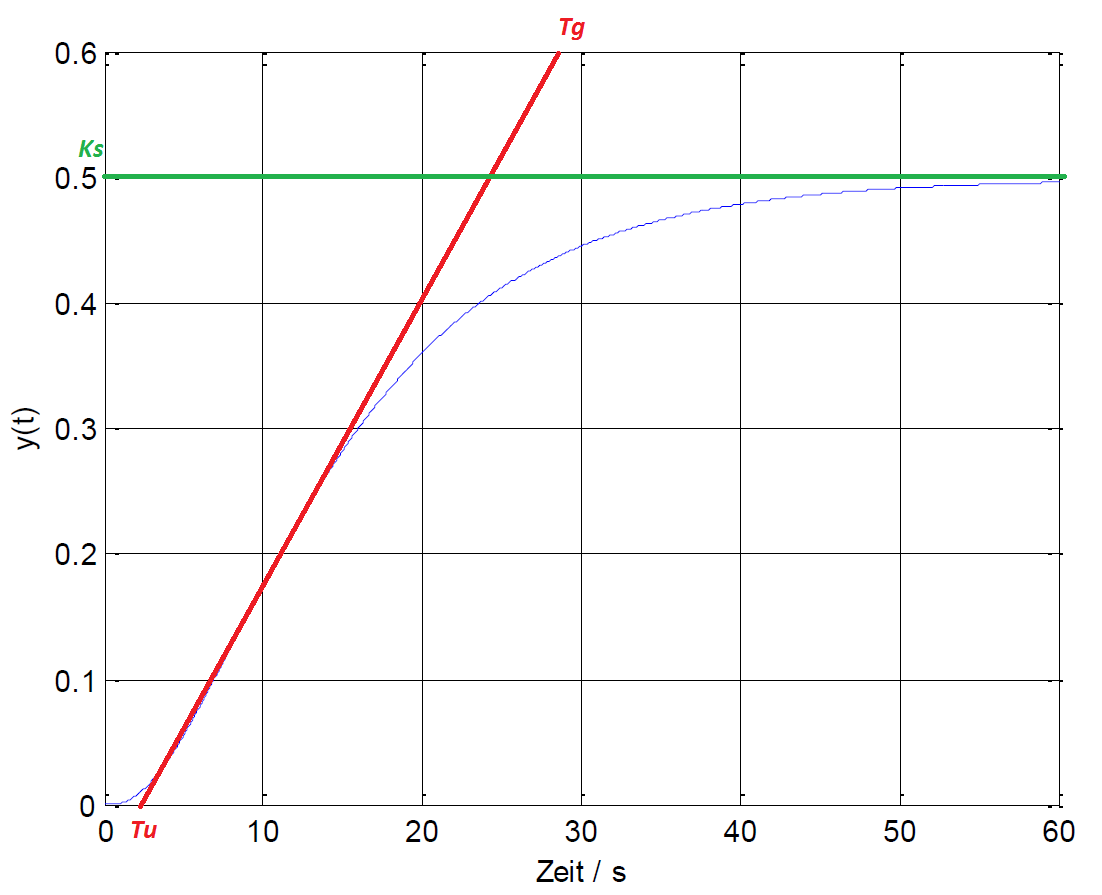
\includegraphics[width=0.5\textwidth]{./Wendetangente.png}
\caption{Regler und Regelstrecke\cite{WendetangenteAuftraggeber}}
\label{fig:Wendetangente}
\end{figure}

Mithilfe dieser Werte und der Sani Methode, welche vom Auftraggeber in Form eines Matlab-Files zur Verf�gung gestellt wurde, ist es einem nun m�glich, die Ordnung der Strecke sowie die Zeitkonstanten $T1$ bis $Tz$ zu berechnen, wobei $Z$ die Ordnung der Strecke ist. Diese Zeitkonstanten werden schlussendlich dazu verwendet die �bertragungsfunktion $H(s)$ zu berechnen:

\[
s=j\cdot w
\]

\begin{equation}\label{�bertragungsfunktion}
H(s)=\prod\limits_{i=1}^Z \frac{1}{(1+s\cdot T_{i})}
\end{equation}

F�r die �bertragungsfunktion eines PI/PID Reglers gilt es zu beachten, dass es zwei Darstellungsarten gibt, die Reglerkonforme, sowie die Bodekonforme. Diese sehen wie folgt aus: \\


PI Reglerkonform:

\[
G_{R}(s) = K_{R}\left(1+\frac{1}{s\cdot Tn}\right)
\]

PI Bodekonform:

\[
G_{R}(s) = K_{R}\left(\frac{1+s\cdot Tn}{s\cdot Tn}\right)
\]

PID Reglerkonform:

\[
G_{R}(s) = K_{R}\left(1+\frac{1}{s\cdot Tn}+\frac{s\cdot Tv}{1+s\cdot Tp}\right)
\]


PID Bodekonform:

\[
G_{R}(s) = K_{RK}\left(\frac{(1+s\cdot Tnk)(1+s\cdot Tvk)}{s\cdot Tnk(1+s\cdot Tp)}\right)
\]

Auf die Verwendung dieser Funktionen sowie deren Herleitung wird im Kapitel \ref{ZellwegerMethode}, Zellweger Methode sowie auch im Anhang \ref{Bodekonf} genauer eingegangen.
%\end{document}
